\secnumbersection{Estado del Arte}
\hlabel{sec:2}

A pesar de que, como fue mencionado anteriormente, AMD ROCm es una plataforma de desarrollo relativamente nueva, esto no ha detenido a diferentes investigadores de comenzar a utilizarla como forma de ampliar el hardware en el que se experimentan diferentes descubrimientos o trabajos científicos.

\subsection{ACELERACIÓN DE FACTORIZACIÓN SVD GPGPU}

En el año 2017, diferentes académicos de la Universidad de Tennessee, la Universidad de Manchester y el Laboratorio Nacional de Oak Ridge junto a un ingeniero de AMD trabajaron en la creación de rutinas BLAS de nivel 1, 2 y 3 para ser aplicadas en la aceleración de problemas pequeños de álgebra linear \cite{svd}.

El resultado final de dichas rutinas entregó una variación de la librería MAGMA, llamada MAGMA \textit{batched routines}, la cual corresponde a software sobre operaciones de álgebra linear optimizado a su uso en GPUs haciendo uso de operaciones por lotes, las cuales promueven la reutilización de datos, la minimización de operaciones y la maximización de ancho de banda.
La razón de utilizar la factorización SVD como modelo de pruebas, fue su gran cantidad de usos en aplicaciones tanto matemáticas como informáticas. 
Además, el uso particular de la versión bi-diagonal de la factorización, se debe 
a que esta se conforma por tres fases: de reducción, de solución y de transformación de vuelta, dentro de las cuales la primera corresponde a un 70\% o 90\% del tiempo total de computo, solo en operaciones de tipo BLAS.

El trabajo realizado se ejecutó finalmente en una GPU NVIDIA K420c GPU, para después portarse con la versión de HIP de aquel entonces a una GPU AMD Fiji Nano. Las características de cada una se ven en la tabla 1.

\begin{table}[h]
\centering
\caption{Descripción técnica de GPUs utilizadas en la aceleración de rutinas BLAS por lote.}
\begin{tabular}{cccc}
\hline
GPU       & \begin{tabular}[c]{@{}c@{}}Ancho de banda\\ {[}GB/s{]}\end{tabular} & \begin{tabular}[c]{@{}c@{}}Rendimiento máximo sobre DP\\ {[}Gflop/s{]}\end{tabular} & \begin{tabular}[c]{@{}c@{}}Tamaño de memoria\\ {[}GB{]}\end{tabular} \\ \hline
K40c      & 288                                                                 & 1430                                                                                & 12                                                                   \\
Fiji Nano & 512                                                                 & 512                                                                                 & 4                                                                    \\ \hline
\end{tabular}
\end{table}

Como se observa, la GPU de AMD (Fiji Nano) es inferior a la de NVIDIA (K40c) tanto en su rendimiento sobre operaciones de doble precisión (DP) como en el tamaño de su memoria, superando únicamente en la velocidad de escritura o lectura a su contra parte.
A pesar de esto, los resultados de las ejecuciones en ambas tarjetas para operaciones GEMV por lotes de tamaño 1000 sobre matrices cuadradas de tamaño progresivo tuvo resultados mucho más altos para la GPU de AMD, llegando a fluctuar entre 80 y 100 [Gflop/s] máximos, en comparación a la estabilización en 40 Gflop/s de la GPU de NVIDIA.

\begin{figure}[h]
\centering
\begin{subfigure}{.5\textwidth}
  \centering
  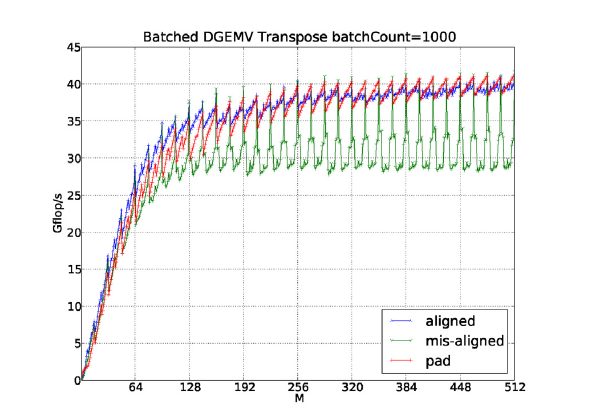
\includegraphics[width=.8\linewidth]{Figures/grap11.png}
  \caption{NVIDIA K40c}
\end{subfigure}%
\begin{subfigure}{.5\textwidth}
  \centering
  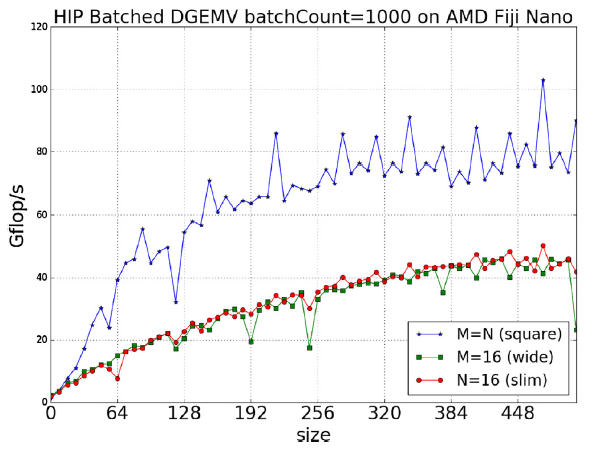
\includegraphics[width=.8\linewidth]{Figures/grap12.png}
  \caption{AMD Fiji Nano}
\end{subfigure}
\caption{Operaciones por segundo en la implementación de MAGMA con lotes de tamaño 1000 sobre matrices cuadradas de tamaño variable.}
\label{fig:4}
\end{figure}

\subsection{USO DE MOTORES DE INFERENCIA JUNTO AL FRAMEWORK \textit{FAST} PARA APLICACIONES MÉDICAS}

Durante el año 2019, un equipo de trabajo conformado por científicos investigadores del instituto médico tecnológico SINTEF en Noruega decidió desarrollar un software para su uso en diferentes aplicaciones médicas. 
Este estaba conformado por un variado conjunto de motores de inferencia, los cuales incluían 5 plataformas de trabajo sobre redes neuronales convolucionales: OpenVino 2019 R1, TensorRT y TensorFlow en tres versiones, sobre CPU, GPU NVIDIA (con cuDNN) y GPU AMD (con ROCm). Además, el equipo utilizó el framework FAST para visualización de imágenes y generación de una interfaz gráfica de aplicación \cite{fast}.

El software final, tiene 3 casos de prueba principales:
\begin{itemize}
    \item Segmentación en tiempo real de imágenes de ultra sonido; el cual corresponde a la localización de segmentos relevantes sobre un flujo grande de imágenes de ultra sonido, normalmente en blanco y negro y con ruido en su señal.
    \item Segmentación volumétrica de tomografías computarizadas; en el que se busca realizar una fragmentación sobre imágenes 3D resultantes de tomografías.
    \item Clasificación sobre parches de microscopía virtual; en donde se espera realizar clasificación de patrones en imágenes generadas por microscopio, cuya resolución ronda los 100k x 200k píxeles y su tamaño aproxima los 56 Gigabytes de datos.
\end{itemize}

En dichos casos, se realizaron diversas pruebas respecto al tiempo de ejecución de cada uno en todos los motores de inferencia que se utilizaron para la generación de la aplicación. 
Para el caso del uso de TensorFlow y TensorRT (desarrollado por NVIDIA para la generación de motores de inferencia sobre GPUs de la misma marca) se utilizó la tarjeta gráfica AMD Radeon R9 Fury para trabajar con ROCm y NVIDIA GTX 1080 ti para CUDA. 
En términos de las pruebas realizadas por caso, no se pudo realizar la segunda sobre segmentación volumétrica en tomografías sobre TensorFlow en ROCm por problemas de la versión de aquel entonces sobre el entrenamiento y evaluación de redes con convoluciones en 3D.
Las características principales de ambas GPUs y los resultados de los demás casos se pueden observar en las tablas 2 , 3 y 4 respectivamente.

\begin{table}[h]
\centering
\caption{Descripción técnica de GPUs utilizadas en implementación de software médico conformado por motor de interferencia más framework FAST.}
\begin{tabular}{cccc}
\hline
GPU         & \begin{tabular}[c]{@{}c@{}}Ancho de banda\\ {[}GB/s{]}\end{tabular} & \begin{tabular}[c]{@{}c@{}}Rendimiento máximo sobre DP\\ {[}Gflop/s{]}\end{tabular} & \begin{tabular}[c]{@{}c@{}}Tamaño de memoria\\ {[}GB{]}\end{tabular} \\ \hline
GTX 1080 ti & 288                                                                 & 1430                                                                                & 12                                                                   \\
R9 Fury     & 512                                                                 & 512                                                                                 & 4                                                                    \\ \hline
\end{tabular}
\end{table}

\begin{table}[h]
\centering
\caption{Tiempo de ejecución sobre segmentación de imágenes de ultra sonido, desde la carga de datos desde el disco hasta el procesamiento de 177 imágenes en la red neuronal. No incluye renderizado y está basado en 10 ejecuciones por motor de inferencia.}
\begin{tabular}{ccc}
\hline
Motor de inferencia & Procesador            & Tiempo de ejecución total {[}ms{]} \\ \hline
TensorFlow CPU      & Intel i5-4460         & 24193 \(\pm\) 1226                   \\
TensorFlow CUDA     & NVIDIA GTX 1080 ti    & 1547 \(\pm\) 17                      \\
TensorFlow ROCm     & AMD Radeon R9 Fury    & 2364 \(\pm\) 23                      \\
OpenVINO            & Intel HD Graphics 620 & 5898 \(\pm\) 26                      \\
TensorRT            & NVIDIA GTX 1080 ti    & 545 \(\pm\) 22                       \\ \hline
\end{tabular}
\end{table}

\begin{table}[h]
\centering
\caption{Tiempo de ejecución sobre clasificación de secciones en imágenes microscópicas, desde la carga de datos desde el disco hasta el procesamiento de la imagen completa. No incluye renderizado y está basado en 10 ejecuciones por motor de inferencia.}
\begin{tabular}{ccc}
\hline
Motor de inferencia & Procesador            & Tiempo de ejecución total {[}ms{]} \\ \hline
TensorFlow CPU      & Intel i5-4460         & 510564 \(\pm\) 1044                  \\
TensorFlow CUDA     & NVIDIA GTX 1080 ti    & 84684 \(\pm\) 1033                   \\
TensorFlow ROCm     & AMD Radeon R9 Fury    & 102594 \(\pm\) 269                   \\
OpenVINO            & Intel HD Graphics 620 & 581054 \(\pm\) 16304                 \\
TensorRT            & NVIDIA GTX 1080 ti    & 81298 \(\pm\) 180                    \\ \hline
\end{tabular}

\end{table}

A partir de estos resultados, se puede notar que la mayoría de los motores que utilizan como procesados una GPU tienen un tiempo de ejecución menor que aquellos que utilizan una CPU.
Si bien para este caso en particular, la GPU AMD fue sobrepasada por el uso del motor TensorRT, esto puede explicarse a que este corresponde a software desarrollado por NVIDIA específicamente para ser aplicado en inferencias y posee una optimización sobre el trabajo con aprendizaje profundo.

\subsection{PORTABILIDAD DE SOFTWARE SOBRE DINÁMICA MOLECULAR EN GPUS MODERNAS}

Dentro de la ciencia de materiales, se ha desarrollado un tipo de simulación para la representación de diferente conceptos mecánicos sobre diferentes tipos de partículas, la dinámica molecular.
Debido a la gran cantidad de fuerzas involucradas, es que la dinámica molecular es una de las simulaciones que más aplica el concepto de HPC.

El año 2020, un grupo de investigadores de diferentes casas de estudio en Rusia trabajaron respecto a como se comportaba el rendimiento de diferentes librerías de dinámica molecular sobre su transformación o porte desde CUDA a ROCm \cite{molecular}.
Particularmente, en el trabajo entregado solo se realizó dicha operación al programa LAMMPS (del inglés, Large-scale Atomic/Molecular Massively Parallel Simulator), software que permite la visualización del comportamiento de partículas dentro de un dominio limitado.
Si bien se trabajaron otros programas respecto a su rendimiento en las GPUs utilizadas, como HOOMD, GROMACS y OpenMM, estos no fueron portados usando las funcionalidades de ROCm, si no que o simplemente no poseían la capacidad de ser ejecutados por la GPU AMD o solo se transformaron a lenguaje OpenCL, el cual puede ser interpretado por GPUs de AMD, pero al tener un mayor nivel de abstracción no se trabaja de una manera óptima.
Para este experimento, se utilizó la GPU Titan V de NVIDIA y Radeon VII de AMD, cuyas especificaciones se pueden ver en la tabla siguiente.

\begin{table}[h]
\centering
\caption{Descripción técnica de GPUs utilizadas en ejecución de software de simulación computacional de dinámica molecular.}
\begin{tabular}{cccc}
\hline
GPU         & \begin{tabular}[c]{@{}c@{}}Ancho de banda\\ {[}GB/s{]}\end{tabular} & \begin{tabular}[c]{@{}c@{}}Rendimiento máximo sobre DP\\ {[}Gflop/s{]}\end{tabular} & \begin{tabular}[c]{@{}c@{}}Tamaño de memoria\\ {[}GB{]}\end{tabular} \\ \hline
%GTX 1080 ti & 484                                                                 & 354                                                                                & 11                                                                   \\
Titan V & 652                                                                 & 7450                                                                                & 12                                                                   \\
Radeon VII     & 1024                                                                 & 3360                                                                                 & 16                                                                    \\ \hline
\end{tabular}

\end{table}

En las pruebas realizadas, se simuló un liquido utilizando el modelo de potencial de Lennard-Jonnes, con un número de átomos variables desde $N = 55296$ a \(4000000\). Los resultados se pueden ver en el gráfico de la Figura~\ref{fig:5}. En esta, los cuadrados abiertos corresponden al resultado del uso del back-end en HIP de ROCm, mientras que los verdes corresponden al uso de CUDA.

A partir de los resultados encontrados, se concluyó de este trabajo que para la transformación realizada desde la versión de LAMMPS para CUDA hacia una versión ejecutable en AMD, se generaba un tiempo de ejecución por átomo por \textit{time step} del mismo orden de magnitud, dentro del rango entre $2.5 \times 10^{-8}$ y $1.3 \times 10^{-8}$ para un número de partículas $N > 10^6$.

\begin{figure}[ht]
    \centering
    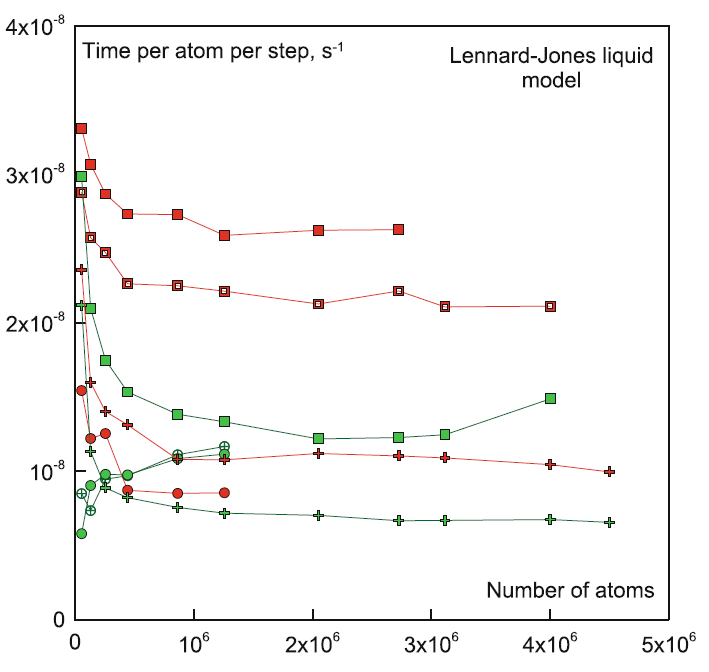
\includegraphics[height=.6\textwidth]{Figures/grap2.png}
    \caption{Tiempo de ejecución por átomo en la simulación computacional de dinámica molecular para un liquido al usar el modelo potencial de Lennard-Jonnes, en [$s^{-1}$].}
    \label{fig:5}
\end{figure}


\subsection{COMPARATIVA DEL SOPORTE EN TIEMPO REAL DE CARGAS EN PYTORCH}

Un equipo de trabajo conformado por académicos de la Universidad de Carolina del Norte en Estados Unidos de América, trabajó sobre la comparativa del rendimiento de diferentes \textit{benchmarks} de la biblioteca PyTorch, utilizado comúnmente para el entrenamiento de redes neuronales en aprendizaje profundo \cite{pytorch}.
Parte del articulo entregado, lista la siguiente serie de ventajas y desventajas del uso de la plataforma ROCm durante el tiempo de desarrollo:

\begin{itemize}
    \item Ventaja 1: El \textit{stack} de software proporcionado por AMD ROCm es \textit{open source} o de código abierto, lo cual implica que el código base esta abierto al publico general para su modificación~\cite{openS}.
    \item Ventaja 2: Programas actualmente presente en CUDA pueden ser transformados a una versión multiplataforma a través de HIP.
    \item Ventaja 3: El software base de bajo nivel en las GPUs AMD permite la partición de los núcleos de sus unidades de computo, lo cual permite una mayor atomicidad en la ejecución y generación de hebras, tanto para renderizado gráfico como para programación general.
    \item Desventaja 1: AMD ROCm solo soporta su uso en sistemas operativos Linux y en GPUs discretas, o las versiones modulares no integradas en placas madres.
    \item Desventaja 2: ROCm esta bajo constantes cambios de gran tamaño, lo cual se debe a su proceso actual de desarrollo.
    \item Desventaja 3: No hay una fuente de documentación oficial y centralizada de la plataforma, lo cual se conforma por cientos de miles de lineas de código.
\end{itemize}

A pesar de estos inconvenientes encontrados, el equipo no tuvo problemas en poder modificar el código de ROCm con tal de poder modificar la cantidad de unidades de computo asignado a las distintas colas de operaciones asignadas a y por la GPU.
Al parecer, este cambio de software de bajo nivel no es posible de implementar para la ejecución en NVIDIA, pues las GPUs de dicha marca no soportan el cambio de tamaño en las ``mascaras'' de unidades de computo a nivel de hardware.
Lo anterior serviría para poder limitar el poder de computo asignado a cada hilo generado.

Por último, para poder generar una comparativa del rendimiento generado por distintas GPUs, se corrió una red neuronal con pesos asignados por un entrenamiento previo con tal de clasificar imágenes de dígitos escritos a mano del conjunto de datos MNIST.
En esto, se utilizaron las GPUs NVIDIA Titan V, GTX 1060, GTX 970, AMD RX 570 y una CPU Intel Xeon 4110, cuyos tiempos de computo y especificaciones (de las tarjetas gráficas) se detallan en la tabla 6 y 7 respectivamente.

\begin{table}[h]
\centering
\caption{Tiempo de computo en la ejecución de una red neuronal para la clasificación de imágenes del conjunto de datos MNIST en [ms].}
\begin{tabular}{cccccc}
\hline
          & Mínimo & Máximo & Media & Promedio & Desviación Estándar \\ \hline
Titan V   & 0.51   & 5.79   & 0.51  & 0.52     & 0.08                \\
GTX 1060  & 1.40   & 1.63   & 1.42  & 1.42     & 0.01                \\
GTX 970   & 1.38   & 2.77   & 1.40  & 1.40     & 0.02                \\
RX 570    & 4.19   & 5.02   & 4.21  & 4.32     & 0.18                \\
Xeon 4110 & 5.54   & 18.43  & 8.60  & 8.40     & 1.78                \\ \hline
\end{tabular}

\end{table}

\begin{table}[h]
\centering
\caption{Descripción técnica de GPUs utilizadas en la ejecución de una red neuronal para la clasificación de imágenes del conjunto de datos MNIST.}
\begin{tabular}{cccc}
\hline
GPU         & \begin{tabular}[c]{@{}c@{}}Ancho de banda\\ {[}GB/s{]}\end{tabular} & \begin{tabular}[c]{@{}c@{}}Rendimiento máximo sobre DP\\ {[}Tflop/s{]}\end{tabular} & \begin{tabular}[c]{@{}c@{}}Tamaño de memoria\\ {[}GB{]}\end{tabular} \\ \hline
Titan V & 652                                                                 & 7.45                                                                                & 12                                                                   \\
GTX 1060 & 192                                                                 & 0.132                                                                                & 6                                                                   \\
GTX 970 & 224                                                                & 0.122                                                                                & 4                                                                   \\
RX 570     & 224                                                               & 0.318                                                                              & 4                                                                    \\ \hline
\end{tabular}

\end{table}

Cabe destacar que si bien los resultados anteriores reportan un menor rendimiento de la GPU AMD RX 570 en perspectiva con las GPUs de NVIDIA, esto se debe netamente al proceso activo de mejoras de la plataforma ROCm, pues en términos de características del hardware, esta está al mismo nivel que la NVIDIA GTX 1060.

En paralelo a los ejemplos de implementaciones realizadas para ambas marcas de tarjeta gráfica con tal de realizar una comparativa en rendimiento, no se pudo encontrar una investigación o caso de prueba que implemente específicamente el método de Lattice Boltzmann y que se ejecute al menos en una tarjeta AMD usando la plataforma ROCm.



